%----------------------------------------------------------------------------------------
%	ARTICLE CONTENTS
%----------------------------------------------------------------------------------------

\section{Introduction}

  Le surpoids et l'obésité se définissent comme une accumulation anormale ou
  excessive de graisse corporelle qui représente un risque pour la santé.

  Le surpoids et l'obésité sont des facteurs de risque majeurs pour un certain
  nombre de maladies chroniques, parmi lesquelles le diabète, les maladie
  cardio-vasculaires et le cancer. \cite{OMS}

  \subsection{Contexte}

  L'agence santé publique France a lancé un appel à projets pour trouver des
  idées innovantes d'applications en lien avec l'alimentation. Nous répondons
  donc à cet appel à projets avec une idée d'application pour smartphone,
  permettant sur base des informations nutritionnelles de proposer des
  produits équivalents à ceux désirés par le consommateur mais avec de meilleurs
  propriétés nutritionnelles.
%------------------------------------------------

\section{Objectifs}

L'objectif principal est d'étudier la faisabilité d'une telle application. Pour
ce faire, une analyse minitieuse des données contenues dans la base de données
d'openfoodfacts est nécessaire. Il s'agit dans un premier temps de cerner les
variables nécessaires au fonctionnement de l'application et ensuite vérifier
que les données permettent bien de répondre à la problématique.

\section{Problématique}

La problématique est double :\newline
La première chose est de s'assurer que les données dont on dispose contienent
bien les informations nécessaires pour créer une telle application.\newline
La deuxième chose :\newline
Peut-on trouver dans la base de données, un produit équivalent avec
de meilleurs propriétés nutritionnelles à partir d'un produit scanné dans
un magasin?

\section{Démarche}

  Pour répondre à la problématique, on se base sur la base de données
  d'openfoodfacts (à l'heure actuelle la plus grosse base de produits alimentaire).
  Une fois les données téléchargées, ces dernières subissent un nettoyage.
  On réalise alors une analyse statistique descriptive
  sur une sélection de variables d'intérêt.
  L'analyse statistique est divisée en deux parties, les analyses univariées et
  les analyses bivariées.

  \subsection{Outils}

    \subsubsection{Matériel}

    L'analyse a été réalisée sur un ordinateur personnel
    (processeur intel i7 4 coeurs, 16 Go de RAM.) et ne nécessite pas de
    matériel particulier.

    \subsubsection{Logiciels}

    L'analyse a été réalisée avec le language Python et des notebooks Jupyter
    sont disponibles dans le répertoire Github (voir section ~\ref{Liens})

\section{Les données utilisées}

  \subsection{Généralités}

  Les données utilisées sont disponibles gratuitement auprès d'Openfoodfacts et
  sont publiées sous licence "Open Database License".

  Les données sont entrées par les utilisateurs (Applications mobiles :
  Openfoodfacts et Yuka). Par conséquent les données sont régulièrement mal
  complétées ou erronées.
  La base de données est assez conséquente (2.2 Go), elle contient (à l'heure
  actuelle\footnote{Novembre 2019}) 1 054 801\footnote{600 654 pour les pays francophones (France,
  Suisse, Belgique et Luxembourg)} d'entrées et 177 colonnes.

  \subsection{Contenu de la base de données}

  Les champs sont séparés en quatres sections:
  \begin{itemize}
    \item Les informations générales sur la fiche du produit: nom, marque, date de création...
    \item Un ensemble de tags: catégorie du produit, localisation, origine, etc.
    \item La liste des ingrédients et les additifs éventuels.
    \item Des informations nutritionnelles: quantités au 100g (graisse, sucre, etc.).
  \end{itemize}

  \subsection{Nettoyage de la base de données}

    \subsubsection{Données concernant la France}
    On ne récupère que les données pour la France et les pays limitrophes
    francophones.

    \subsection{Taux de remplissage des champs}

    On peut regarder le taux de remplissage des champs de manière graphique à
    l'aide d'un graphique type matrice. (chaque valeur est alors représentée
    par un tiret (les colonnes noires sont alors totalement complètes et les
    colonnes vides sont blanches.) Voir graphique \ref{completion_field}

    \begin{figure*}[b]
      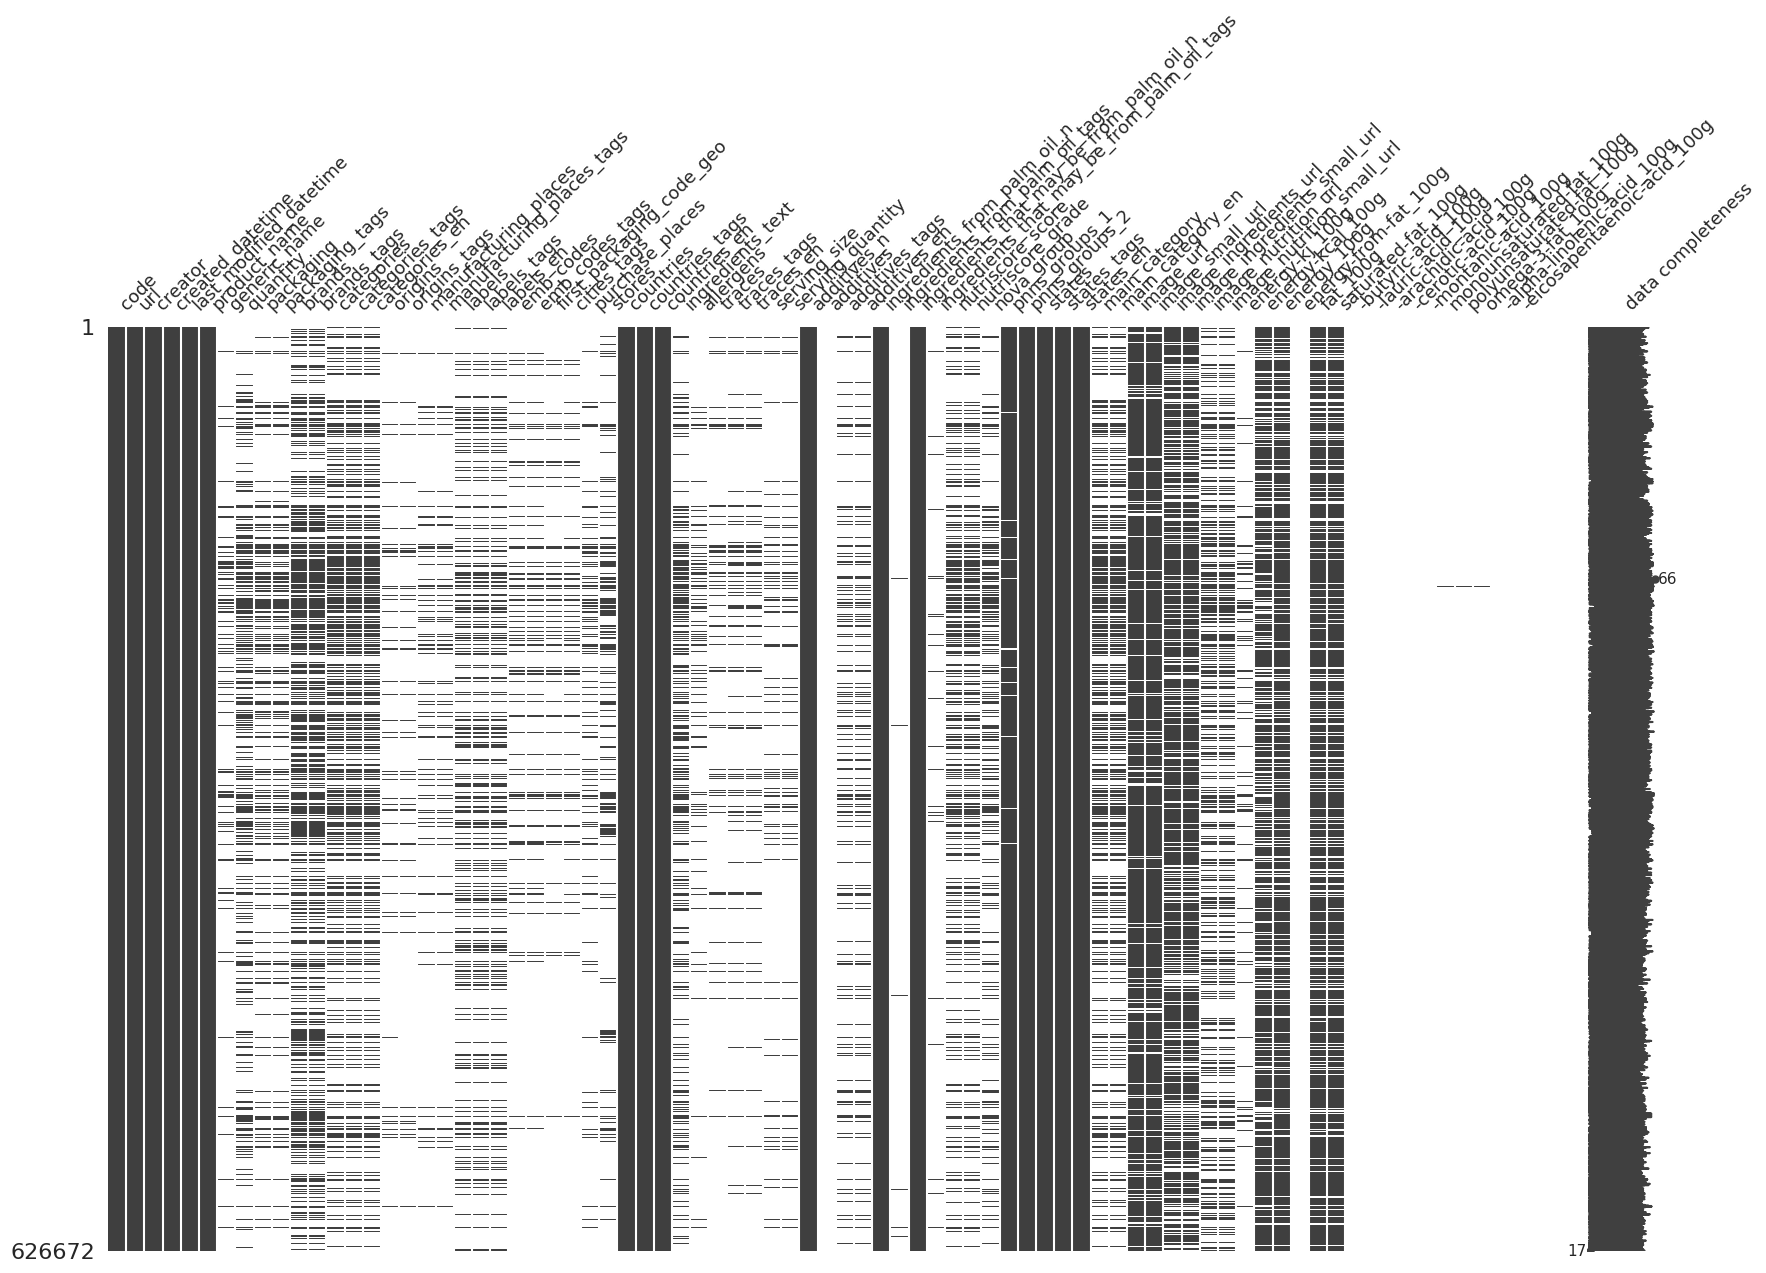
\includegraphics[width=\linewidth]{completness_part_1.png}
      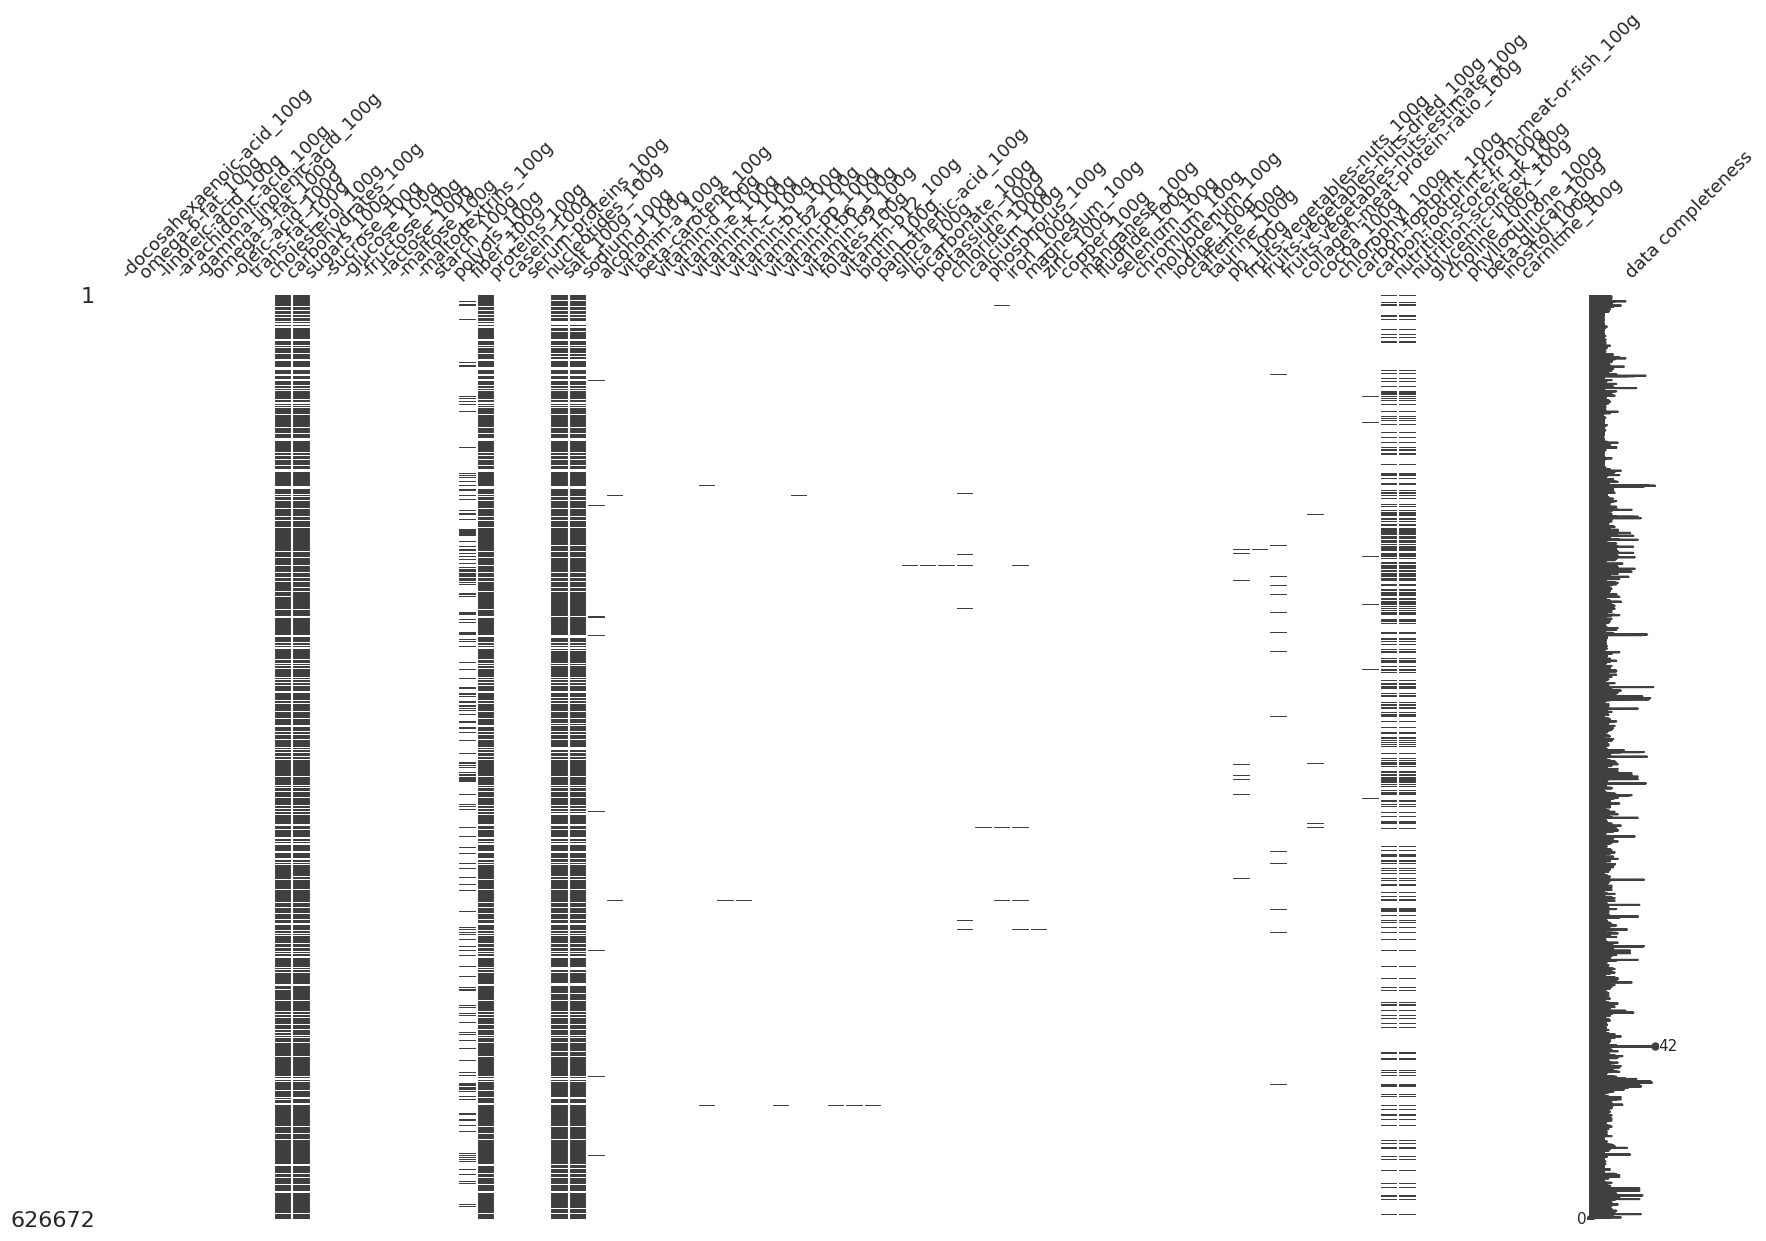
\includegraphics[width=\linewidth]{completness_part_2.png}
      \caption{Taux de remplissage des variables. En haut les colonnes de 1 à 78
      et en bas le reste des colonnes. Les colonnes vides ont été retirées}
      \label{completion_field}
    \end{figure*}

    On peut regarder la distribution du nombre de champs complétés.
    \begin{figure}[H]
      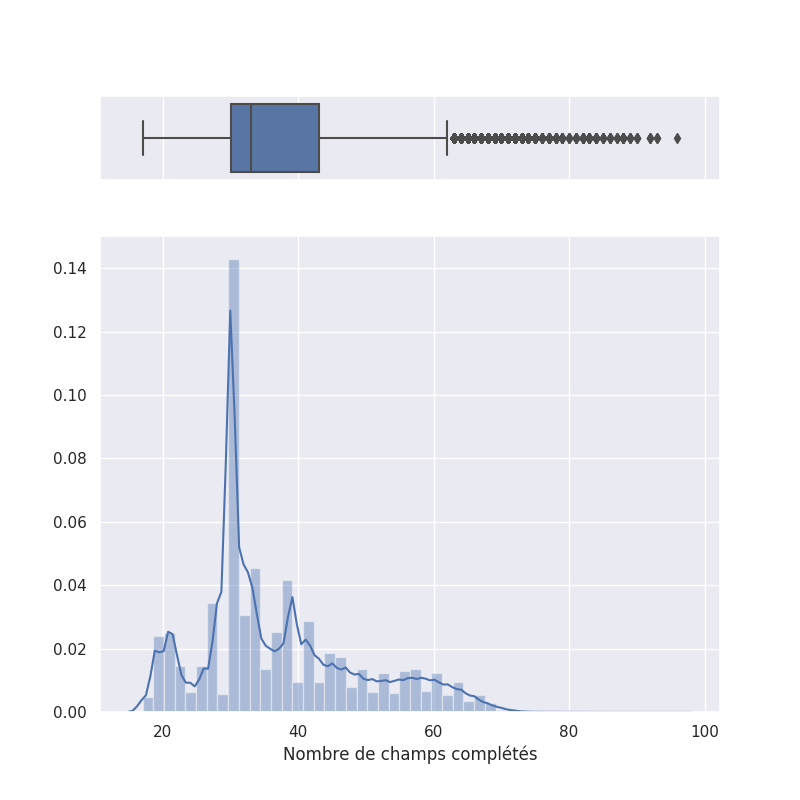
\includegraphics[width=70mm]{nombre-de-champs-completes-dist.png}
      \caption{Distribution du nombre de champs complétés.}
      \label{distrib_completion}
    \end{figure}
    On a au minimum 18 champs complétés et 97 champs complétés maximum.

\section{Analyses univariées}

  \subsection{Variables sélectionnées}
  Pour assurer la faisabilité du projet, nous avons besoins de :
  \begin{itemize}
    \item Le nom du produit
    \item Le code bar du produit
    \item La marque du produit
    \item La catégorie à la quelle appartient le produit
    \item Le nutriscore (nutrition grade [A, ..., E])
    \item Certaines données nutritionnelles :
    \begin{itemize}
      \item Valeur énergétique au 100g
      \item Teneur en protéines
      \item Teneur en sucres
      \item Teneur en graisses
      \item Teneur en sel
    \end{itemize}
  \end{itemize}
  \subsection{Répartition du nutriscore}
  \begin{figure}[H]
    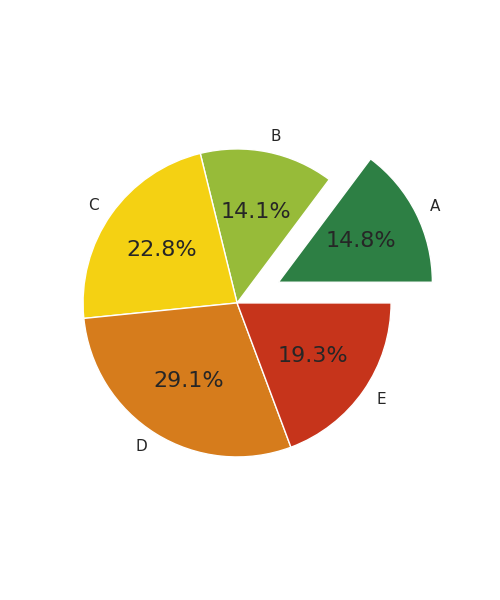
\includegraphics[width=70mm]{nutriscore-repartition.png}
    \caption{Répartition du nutriscore des produits}
    \label{nutriscore_pie}
  \end{figure}

  \subsection{Valeurs énergétiques des produits}
  \begin{figure}[H]
    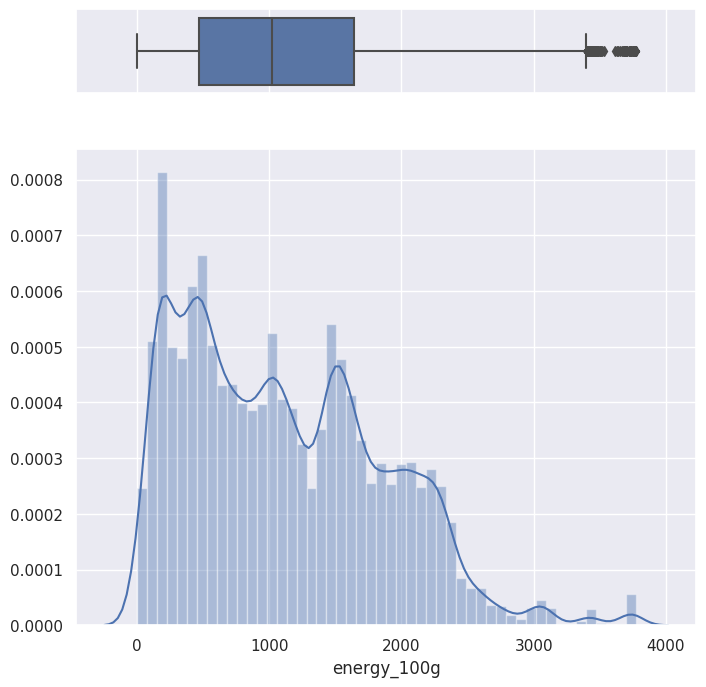
\includegraphics[width=75mm]{distribution_valeur_energetique.png}
    \caption{Distribution des valeurs énergétiques des produits dans la base
    de données.}
    \label{}
  \end{figure}
\section{Analyses multivariées}
Toujours dans l'objectif de trouver un produit équivalent, il est important
de vérifier que pour chaque catégorie (ici groupe Programme nutrition santé PNS)
il existe des produits pour chaque nutriscore (de A à E).

\section{Conclusion}

\section{Perspectives}

%\section*{Remerciements}

\section{Liens internet}
\label{Liens}
\begin{itemize}
  \item \faGithub \url{https://github.com/tgrandjean/OC-sante-publique-france}
  \item \faDatabase \url{https://world.openfoodfacts.org/data}
\end{itemize}
